\documentclass[conference]{IEEEtran}
%\documentclass[10pt,sigconf,letterpaper]{acmart}

%\renewcommand\footnotetextcopyrightpermission[1]{} % 
%removes footnote with conference info
%\setcopyright{none}
%\settopmatter{printacmref=false, printccs=false, 
%printfolios=false}
%\pagestyle{plain}


\usepackage{color}
%\usepackage[nolist]{acronym}
%\usepackage{amsmath,amssymb}
\usepackage{pifont}
%\usepackage{enumitem}
\usepackage{booktabs}
\usepackage{url}
\usepackage{xcolor}
%\usepackage{times}  % Times fonts look better
\usepackage{array}  % Extended styles for tables
\usepackage{textcomp}
\usepackage{cite}
\usepackage{amsmath,amssymb,amsfonts}
\usepackage{algorithmic}
\usepackage{graphicx}
\usepackage{textcomp}
\def\BibTeX{{\rm B\kern-.05em{\sc i\kern-.025em b}\kern-.08em
		T\kern-.1667em\lower.7ex\hbox{E}\kern-.125emX}}

% \iffalse
\iftrue
\newcommand{\randall}{\ding{110}\ding{43}\textcolor{magenta}}
\newcommand{\pes}{\ding{110}\ding{43}\textcolor{blue}}
\newcommand{\geoff}[1]{\ding{110}\ding{43}\textcolor{violet}{#1}}
\else
\newcommand{\randall}{}
\newcommand{\geoff}[1]{}
\fi

%\DeclareFontFamily{\encodingdefault}{\ttdefault}{\hyphenchar\font=`\-}

% \setcopyright{acmcopyright}
% \copyrightyear{2018}
% \acmYear{2018}
% \acmDOI{10.1145/1122445.1122456}

%\copyrightyear{2022}
%\acmYear{2022}
%\acmConference[IMC '22]{Internet Measurement 
%Conference}{October 25--27, 2022}{Nice, France}
%\acmConference{}{}{}
%\acmBooktitle{Internet Measurement Conference (IMC '22), 
%October 25--27, 2022, Nice, France}
%\acmPrice{TBA}

\begin{document}

\author{Anonymous Authors}
%\author{Audrey Randall}
%\email{aurandal@eng.ucsd.edu}
%\affiliation{UC San Diego}
%\author{Peter Snyder}
%\email{pes@brave.com}
%\affiliation{Brave Software}
%\author{Alisha Ukani}
%\email{aukani@ucsd.edu}
%\affiliation{UC San Diego}
%\author{Alex Snoeren}
%\email{snoeren@cs.ucsd.edu}
%\affiliation{UC San Diego}
%\author{Geoffrey M.\ Voelker}
%\email{voelker@cs.ucsd.edu}
%\affiliation{UC San Diego}
%\author{Stefan Savage}
%\email{savage@cs.ucsd.edu}
%\affiliation{UC San Diego}
%\author{Aaron Schulman}
%\email{schulman@cs.ucsd.edu}
%\affiliation{UC San Diego}

\title{The Challenges Associated With Decentralized Naming for Legal Takedowns}
%\renewcommand{\shortauthors}{A. Randall \textit{et al.}}

%\runningtitle{Article title}

%\subtitle{...}

%\abstract{stuff?}


\maketitle
\pagestyle{plain}

\section{Introduction}

%\begin{itemize}
%	\item Malware, particularly botnets (any other types? ransomware?) 
%	uses DNS to reach CNC 
%	servers. 
%	\begin{itemize}
%		\item Malware needs a naming layer because of the 
%		sunk infrastructure cost: 
%		any malware already deployed that uses an IP that gets blocked/taken 
%		over is now useless. Malware authors want a record they can change.
%		\item Naming layer needs to be hard to block at both 
%		the request level and the system level, so that 
%		already-distributed malware doesn't lose access and 
%		become useless. 
%	\end{itemize}
%	\item DNS is decentralized in that there are many resolvers, but 
%	centralized in that there are centralized authorities. Defenders can serve 
%	legal takedown notices to those centralized authorities to block malware's 
%	access to its CNC servers.
%	\item Pivot: Malware is starting to use a truly decentralized naming 
%	system, ``blockchain DNS.'' This creates several challenges for defenders:
%	\begin{itemize}
%		\item No central authority is capable of enacting domain-level takedown 
%		orders
%		\item For large chains, there is enough legitimate content that 
%		blocking access to the whole chain is infeasible
%		\item Transactions on large chains cost a lot of money. This limits 
%		defenders' abilities to stage interventions like pre-registering all 
%		domains listed in a malware's DGA.
%	\end{itemize}
%	\item We study the ecosystem and point out several places where 
%	interventions are still possible, and discuss the challenges to defenders 
%	and occasional advantages they gain when malware uses decentralized naming 
%	such as blockchain DNS.
%\end{itemize}

Malware that is distributed across multiple machines needs a way to distribute commands, upload stolen 
data, and coordinate between infected hosts. Most malware, such as botnets or ransomware, uses a 
central command and control (C2) server for this task. However, as a single point of failure, a 
central C2 server presents an obvious weak link for defenders to target 
~\cite{kesari_deterring_2017}. 
Malware authors must therefore be able to easily relocate and replace a C2 server after a defender 
takedown. All previously infected hosts must be able to find the new server at its new address, 
without outside coordination --- if they cannot, they become useless. Malware authors avoid 
this ``sunk cost'' problem by providing a layer of indirection --- a naming layer --- instead of 
hard-coding a fixed C2 server address directly into deployed malware. This naming layer must be 
resilient to takedown efforts.

Until recently, the naming layer used most frequently by malware was ordinary DNS, which is rarely 
blocked at the protocol level, universally supported, and easy to configure. Malware authors use 
various strategies, such as fast flux or DGAs (domain generation algorithms), to cycle through domains 
or the IP addresses they resolve to and complicate defense efforts. However, DNS domains are subject 
to central authorities, who may be compelled to seize or deny access to abused domains. Malware 
authors have recently come up with an innovative solution to this risk: they have started to use 
\emph{decentralized naming systems}, in particular naming systems built on blockchains. 

Decentralized naming systems present several potential challenges for defenders. First, because they 
have no central authority to carry out legal takedown requests, decentralized systems are immune to 
one of the most effective tools in malware defenders' arsenals. Second, some decentralized systems 
have high transaction costs to register and manage domains, which renders certain existing defender 
strategies less effective. For example, registering all domains that a DGA might eventually generate 
is impractical in expensive decentralized naming systems. However, decentralized naming systems 
present challenges to malware authors as well, such as how to stealthily access the system.

We study the ecosystem and point out several places where defender interventions are still possible. 
In particular, we argue that infected hosts must pass through infrastructure that is at least 
partially centralized to access any fully decentralized naming system, and these centralized or 
partially centralized ``chokepoints'' still present viable points to stage interventions. We also 
study five existing decentralized, blockchain-based naming systems, and discuss the challenges and 
advantages that each present to malware authors and defenders. We conclude that which decentralized 
naming systems present a significant threat, defenders still have viable options for enacting C2 
takedowns.

The remainder of this paper is organized as follows...

\section{Background}

From a malware author's perspective, an ideal naming system for C2 
addresses must be uncensorable at both the request level and the system level. To be 
uncensorable at the request level, there should be no central authority that 
has the ability to enforce a legal takedown notice for an individual record. To 
be uncensorable at the system level, the system should be valuable enough to 
licit actors that authorities cannot block access to it entirely without 
causing significant collateral damage to benign users.

To some extent, a trade-off exists between these features. On 
one side of the 
spectrum, protocols like Tor provide high resistance to request-level 
censorship, but they stand out in network traffic, allowing systems like 
IDSes to detect the 
malware's presence. For example, enterprise networks often block Tor 
entirely under the assumption 
that none of their employees will use it for any legitimate purpose.
%but do not have enough licit traffic to prevent authorities from 
%blocking access to the system entirely. \randall{Cite that paper that   
%said when you take away the malware, what's left is 80\% CSAM, and find other 
%citations that say defenders block Tor.}
On the other side of 
the scale, malware has repurposed ubiquitous, benign systems 
such as social media to store C2 addresses. Defenders do not 
want to impose blanket bans on applications accessing social 
media URLs, but social media companies such as Facebook and 
Twitter have the capability, motivation, and legal obligation to enforce 
legal takedown requests on individual posts. Malware authors want to use 
systems that are balanced 
between being difficult to block at the record level and difficult to detect 
and block at the 
system level.

\subsection{DNS-based domain names}

Traditional DNS has high system-level resistance to censorship but low 
request-level resistance. 
Since nearly every device and application on the Internet requires DNS, 
enterprises and firewalls 
almost never block it entirely. However, while DNS is a decentralized 
system in terms of how its 
components are replicated across the globe, it is not decentralized in terms 
of authority. The 
registrar that sold a domain can be compelled to ``delete'' that domain or 
prevent it from being 
updated or transferred. 

The usual process for enacting a legal takedown in the United States works as 
follows~\cite{knight_domain_2015}. Upon 
identifying a domain that is being used as a C2 center, a law enforcement 
entity may choose to make 
an Acceptable Use Policy (AUP) complaint or may immediately seek a court order 
compelling the 
registrar to take down the domain. Some registrars cooperate with AUC 
complaints without legal 
intervention, but others do not. If the registrar does not respond to the 
AUC complaint and take 
down the domain, law enforcement may move on to using a court order. The 
court order commonly 
prevents the domain from being updated or transferred rather than deleting it 
entirely, because if 
the domain is deleted, it can be re-registered by the malware authors. The 
court order also 
specifies whether the domain should continue to resolve, resolve to a new IP 
address specified by 
the order, or stop resolving altogether. 

Court orders may be obtained by civil parties as well. The most common method 
is for a company to 
apply for a temporary restraining order (TRO), which orders the perpetrators 
of the offending 
activity to cease and desist and requires any intermediaries that provide 
services to the 
perpetrators to cease providing those services~\cite{kesari_deterring_2017}. 
The latter requirement 
is what allows companies to require registrars to ``sinkhole'' C2 
domains. 

Legal domain takedown orders are a critical tool for defenders to disable 
botnets. For example, 
Microsoft obtained various court orders allowing it to sinkhole the C2 servers 
of the botnet 
Citadel in 2013. Microsoft successfully argued that Citadel caused the Windows 
operating system to 
behave maliciously and frustrate users while still bearing Microsoft 
trademarks, as well as forcing 
Microsoft to spend money on security features to combat 
it~\cite{lerner_microsoft_2014}. The 
Coreflood, Kelihos, and Rustock botnets were each disabled using legal 
takedown orders obtained by 
Microsoft, Pfizer (which claimed to suffer reputational harm because Rustock 
sent spam emails for 
counterfeit pharmaceuticals), and the Department of 
Justice~\cite{kesari_deterring_2017}. These 
takedowns are possible because in each case, some centralized entity had 
control of the C2 servers' 
domain names, and thus had the capability to take them down when legally 
compelled to. Malware 
authors are thus incentivized to find naming systems that are not vulnerable to 
legal takedowns.  

\subsection{Blockchain-based domain names}

Blockchain-based naming systems present a potential threat 
because they claim to be immune to takedowns. No central authority 
controls blockchain domains in the same way that registrars 
control traditional DNS names. In general, it is not possible to modify or 
delete a record on a blockchain without controlling the record's private 
key. Once a domain has 
been registered, its ownership is passed to the purchaser, after which 
point even the company that 
sold it cannot modify it. The record is also stored immutably on the 
blockchain for as long as the 
chain exists, even if the owner later modifies or deletes it, because 
historical recods are part of 
the blockchain and cannot be erased. Blockchain-based naming systems 
therefore have high resistance 
to request-level censorship.

Furthermore, some blockchains are popular enough to be challenging to block 
without 
harming licit users. Blockchains such as Bitcoin and Ethereum have recently 
skyrocketed in popularity as investors became interested in cryptocurrency as 
an asset class. Because these blockchains are no longer niche systems used 
only by a few 
technologically-savvy users, blocking access 
to them entirely may be difficult without angering a large number of 
legitimate users. As far as we are aware, cryptocurrencies and the blockchains 
they rely on are the first examples of strongly censorship-resistant systems 
that have gained a substantial community of legitimate users around the world.

Blockchain is therefore an attractive option for malware authors to use as a 
naming 
layer for C2 server addresses. In fact, some malware is already exploiting 
these tools.
BazarLoader uses the Emercoin ``.bazar'' TLD to record the domains of its C2 
servers~\cite{brandt_bazarloader_2021}. The Namecoin TLD 
``.bit'' is used by the
Necurs botnet~\cite{dgas_of_necurs}, the Chthonic banking 
trojan~\cite{malware_traffic_analysis_2016}, Smoke Loader/Dofoil, 
Backdoor.Teamviewer, Shifu, 
and TinyNuke~\cite{abusech_2017, mackie_cryptodns_2018}. Cerber ransomware 
has 
even used blockchain wallet addresses as names for its C2 
servers~\cite{pletinckx_malware_2018}.

However, we find that blockchain domains are not as invincible as they 
claim. While sinkholing 
blockchain domains through their registrars is not possible, blockchain 
domains have two different 
weaknesses that DNS does not have: accessing the system and modifying records.

 Blockchain domains are not accessible through traditional DNS. Instead, 
 malware 
must find a way to contact a member of the blockchain to resolve its chosen 
domain. Malware authors 
can implement this in two ways: they can either use a centralized proxy with a 
known domain to gain 
access to the blockchain, or they can act as first-class participants of the 
blockchain themselves, 
and participate in the peer-to-peer discovery protocol. Both approaches 
present opportunities for 
defenders to intervene. 

Modifying records on blockchains also poses new challenges for both defenders 
and malware authors. 
Modifications are usually more expensive (in terms of money) than in DNS, 
making fast flux or DGA 
impractical on some chains. Similarly, if a defender wishes to register 
all domains that a DGA 
might produce, this becomes expensive on some chains.

In the remainder of this work, we detail the specific challenges posed by the 
blockchain DNS 
ecosystem to malware authors and defenders, as well as the pieces of the 
ecosystem where 
effective interventions might be staged.

\section{Accessing records}

\begin{figure*}[t]
	\centering
	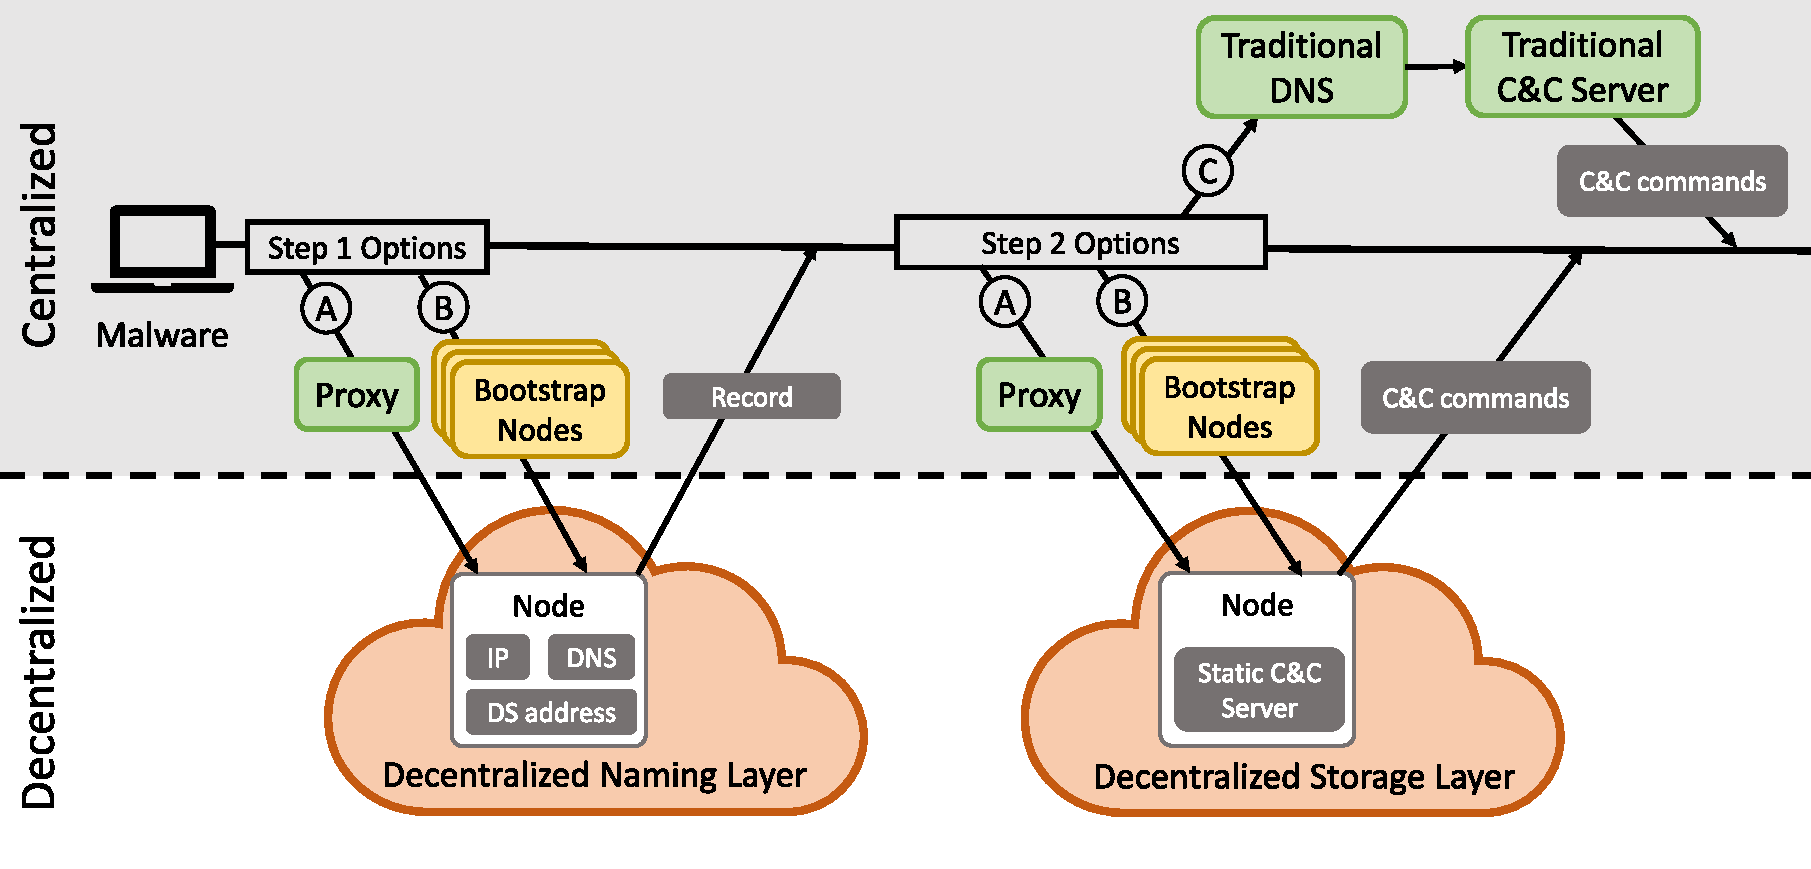
\includegraphics[width=\textwidth]{figs/malware_contacting_cnc.pdf}
	\caption{Malware must pass through centralized ``chokepoints'' to reach 
		decentralized systems, some of which might be good points for defender 
		interventions.}
	\label{fig:malware_contacting_cnc}
\end{figure*}

We have established that malware requires a naming layer to access its C2 
centers, and 
that blockchain-based naming systems are attractive options for implementing 
such a naming layer. 
We will now discuss the fundamental requirements of distributed naming systems 
and how 
these requirements present challenges and advantages to defenders. The first 
such fundamental 
requirement is accessing the distributed system.

To access name records stored on any distributed system like a blockchain, 
infected hosts must 
first obtain access to the blockchain itself. Accessing any distributed, 
peer-to-peer system for 
the first time requires learning the address of at least one participating 
node. In general, there 
are two methods for finding such an address: connecting to a 
proxy that already knows how to reach a member of the system, or acting 
as a full member of the system yourself and utilizing its peer-to-peer 
discovery protocol. The 
latter approach requires knowing a list of ``bootstrap nodes.'' For example, 
Ethereum uses a list 
of bootstrap nodes that are hard-coded into various client 
implementations. Bitcoin 
stores lists of nodes in DNS TXT records maintained by volunteers, as well 
as hard-coded 
lists~\cite{citation_needed}. A third option, a 
local discovery protocol that floods the network with 
messages looking for nodes, has not been adopted by any major 
blockchains that we are aware of. Such an approach would only be successful if 
the nodes running 
the blockchain were ubiquitous. It would also be very ``noisy'' and so 
unlikely to be favored by 
malware, so we do not discuss it further. 
Figure~\ref{fig:malware_contacting_cnc} shows the options 
infected hosts may choose from when connecting to a decentralized naming 
system, which we now 
discuss in more detail.

%Anything in Figure~\ref{fig:malware_contacting_cnc} in green is 
%centralized 
%enough to have to respond to a takedown request. Anything in yellow is 
%more difficult because taking it down would have collateral damage, and in 
%orange it's probably impossible to take down because it's truly 
%distributed and 
%very resilient to takedowns.



\subsection{Accessing blockchains using proxies}

\begin{table}
	\begin{tabular}{r l l}
		\toprule
		Name system & TLDs & Proxies \\
		\midrule
		Namecoin & .bit & BDNS \\
		Emercoin & .lib, & PeerName,  \\
		& .bazar, & friGate, \\
		& .coin, & OpenNIC \\
		& .emc & \\
		Handshake & \emph{any string} & hns.to, \\
		& & NextDNS, \\
		& & HDNS.io,\\
		& & BobWallet extension, \\
		& & LinkFrame extension \\
		ENS & .eth & eth.link, \\
		& & eth.limo \\
		Unstoppable & .crypto, & Brave browser, \\
		& .blockchain, & Opera browser, \\
		& .bitcoin, & Unstoppable browser, \\
		& .coin, & Unstoppable extension, \\
		& .nft, & Infura\\
		& .wallet, & \\
		& .888, & \\
		& .dao, & \\
		& .x, & \\
		& .zil & \\
		\bottomrule
	\end{tabular}
	\caption{Non-exhaustive selection of proxies, browsers, 
	and extensions 
	that can be used to access blockchain-based naming 
	systems. \randall{maybe should have a citation for each 
	of these}}
	\label{tab:proxies_and_tlds}
\end{table}

To resolve a blockchain-based name by using a proxy, users have several 
choices. Most large 
browsers, such as Safari, Chrome, and Firefox, do not support any 
blockchain 
naming systems natively. However, several extensions allow users to resolve 
names from ENS, 
Handshake, and Unstoppable Domains. These extensions rely on proxies that 
use 
DoH to send a resolution request to a server that can resolve the name. We 
note that such a server does not need to make a lookup to the chain every time 
it receives a request: it may cache names or keep track of its own database 
of 
names, which would simplify its implementation and speed up lookups 
significantly. 

Some browsers, such as Brave and Opera, claim to resolve certain naming 
systems 
natively. \randall{but when I tried this it didn't work? should try again 
with 
known websites and try Opera.} Both Brave and Opera rely on a proxy called 
Infura to resolve blockchain-based names. \randall{many citations 
needed.} 

Some naming systems have partnerships with existing DNS resolvers. For 
example, 
NextDNS and Handshake have partnered to allow users who set their DNS resolver 
to NextDNS to resolve Handshake domains. Finally, some naming systems, 
such as 
Handshake, also provide stub resolver implementations that run locally on a 
user's computer. 

As a side note, the existence of competing naming systems in which name 
collisions are possible 
opens up the possibility of collision-based attacks. There is no governance 
system in place to prevent different systems from adopting the same TLDs and 
causing name collisions. In fact, several collisions already exist, both 
between blockchain-based systems themselves (Emercoin and Unstoppable both 
provide a ``.coin'' TLD) and between ICANN TLDs and blockchain-based systems 
(both Handshake and ICANN provide ``.music''). 
This means the record that a user receives when resolving a name with a 
collision depends on which resolution method they use. If the user has 
multiple 
proxies set up --- for example, multiple browser extensions installed that 
each 
try to resolve domains with a specific TLD --- then the record received will 
depend on which of those proxies takes precedence, which is not at all 
clearly 
defined. This lack of centralized governance enables several classes of 
attacks, such as squatting 
and phishing, which are beyond the scope of this paper.

Table~\ref{tab:proxies_and_tlds} provides a summary of the TLDs and 
proxies 
used by the blockchain naming systems we study. The list of proxies is not 
exhaustive, but 
represents 
a subset of the best-known proxies in use at the time of writing.
All of these proxies are 
centralized, which is good news for defenders: similarly to traditional 
registrars, they are vulnerable to legal takedowns. They can be served with 
legal takedown notices and compelled to stop giving access to abused domains, 
as long as they 
operate within a jurisdiction amenable to such efforts. A centralized proxy 
could also be taken 
down entirely by serving a takedown order to its hosting provider. While 
these interventions are 
not bulletproof, they are subject to the same advantages and disadvantages 
as 
interventions on traditional registrars. Thus, centralized proxies return 
the 
distributed naming ecosystem to a state similar to the DNS ecosystem, from a 
defender's point of view. However, while proxies simplify the process of 
connecting to a blockchain, they are not strictly necessary, which is bad 
news 
for defenders.


\subsection{The emergence of light clients}

When blockchains were first envisioned, most assumed that every participant in 
the network would be a ``full'' implementation of a node: it would contain 
enough state to reconstruct the entire history of the chain, all the way back 
to the first transaction. Additionally, each node would contribute to the 
blockchain by verifying every transaction it heard about. As various 
blockchains have grown over time, they have become too resource-intensive to 
run on anything other than a dedicated, powerful machine. Two 
resources serve as 
the constraints: first, CPU power, which is obviously necessary to perform 
mining but now is even a bottleneck for transaction verification on some 
machines, because so many transactions happen per 
second~\cite{citation_needed}. Second, disk 
space and speed. For example, Ethereum cannot be run on a machine with a hard 
disk drive anymore, because nothing slower than an SSD can keep up with the 
reads and writes required~\cite{citation_needed}. \randall{I 
forget where I read this.} These resource constraints have 
given rise to the concept of a ``light client,'' a blockchain 
node with limited functionality that can fetch transactions 
from the chain but does not contribute by verifying 
transactions, mining, or broadcasting. Light clients are 
designed to run on laptops and mobile devices. As 
such, they are small enough to reasonably fit into a malware 
payload. 

Light clients enable malware to act as a first-class member 
of a blockchain, and discover other members of the chain 
using the chain's peer-to-peer discovery protocol without 
using a centralized proxy. Most peer-to-peer discovery 
protocols allow a client to connect to the blockchain for the 
first time by hard-coding a set of ``bootstrap nodes.'' In 
Ethereum, these bootstrap nodes are hard-coded into various 
implementations of the clients, and in Bitcoin, they are 
either hard-coded or accessible as TXT records stored at 
various trusted domains. The list of bootstrap nodes may also 
be configured by the user. If the 
malware chooses to use the bootstrap nodes that are 
hard-coded by default into the light client implementation, 
this may present a challenge for defenders, because taking 
down those bootstrap nodes may cause collateral damage to 
legitimate users attempting to join the chain. As such, 
bootstrap nodes are a more difficult place to stage an 
effective defender intervention than centralized proxies. 

Prohibiting malware from accessing a blockchain by intervening with the 
bootstrap nodes poses challenges compared to staging interventions at 
centralized proxies. If 
defenders take the bootstrap nodes down entirely, they risk causing 
collateral damage, by blocking 
access to the chain for licit users. However, because the IP addresses of 
the bootstrap nodes are 
public, defenders could also choose to add them to blocklists: IDSes, 
enterprise firewalls, or ISP 
routers can drop traffic intended for those destinations. The blocklist 
approach is very similar to 
blocking any other malicious IP addresses, and is subject to the usual 
challenges. Defenders must 
keep blocklists up-to-date as malware authors update the IPs they connect to, 
and malware authors 
could quickly pivot from using published IP addresses to IPs of nodes that they 
run 
themselves which are not publicly known. To the advantage of defenders, 
any time malware authors 
are forced to update the IP addresses that bootstrap nodes may be found at, 
they run 
afoul of the ``sunk cost'' problem where already-deployed malware that cannot 
be updated becomes 
useless. A similar argument applies if malware chooses to access bootstrap 
nodes using hard-coded 
DNS domain names instead of hard-coded IP addresses. Additionally, 
traditional interventions 
against domain names apply in that situation as well. Thus, while 
intervening at bootstrap nodes 
poses more of a challenge than intervening at centralized proxies, defenders 
still have viable 
options available.

\subsection{Naming record formats}

If malware successfully contacts the naming layer, it can then fetch the 
record that allows it to 
access its C2 center. 
This record can take several forms. The three that we observed in existing 
blockchain naming 
systems that might be useful to malware were IP addresses, 
traditional DNS domains, and addresses to distributed file storage 
systems like IPFS and SkyNet. We refer to these addresses as ``distributed 
storage'' (DS) 
addresses. Some naming systems allow users to store arbitrary text as 
records, which would allow 
malware to use nonstandard record types like links to social media posts. 

Each of these record types are subject to all of the traditional interventions 
that have already 
been described, except one: DS addresses. Distributed storage systems 
present a further challenge 
to defenders that goes beyond the challenges of decentralized naming. They 
enable malware authors 
to run an entire C2 center on a blockchain-based system that has no central 
authority capable of responding to a takedown request. In this respect, 
they provide a limited form 
of ``bulletproof'' hosting, and present their own unique challenges for 
both malware authors and defenders.

The decentralized storage systems available today do not offer the ability to 
host dynamic 
websites, so any C2 center implemented entirely on such a system must be a 
simple file with no 
dynamic content. Additionally, today's DS systems are 
content-addressed, which presents a challenge 
for malware authors that wish to hard-code the DS address of their C2 center 
into their payloads. 
If the file that represents the C2 server changes, its address will change as 
well, because the 
address is created from a hash of the file.

Some DS systems do not have redundancy, which raises the possibility of 
discovering the particular 
machine(s) responsible for hosting a C2 server and seizing it. 


\randall{where do I put this? Additionally, because all blockchain 
records 
are public, anyone can fetch those records including 
defenders. You could theoretically scrape a blockchain looking for records 
that match a known 
malicious format or with malicious traits of some sort (owned by the same 
wallet?) and try to seize 
whatever those records point to.} 

Accessing a DS system is the same as accessing a distributed 
blockchain-based naming layer: you can do it either by proxy 
or by being a first-class member of the network, in which 
case you need bootstrap nodes. Theoretically, malware can go 
straight to the storage layer, but this is unlikely to be 
feasible given the way current DS systems are set up. The 
reason malware needs 
to use a naming layer to connect to the current generation of 
distributed file storage systems is because they're 
content-addressable. As soon as the file changes, so 
does its address, and the malware that knew the old address 
is useless. 
However, this is not a fundamental limitation of distributed 
storage systems --- a system could be designed in the future 
that doesn't have this limitation.

I don't know if IPFS/SkyNet have light nodes that could be 
part of a malware payload, but there does seem to be a trend 
in that direction as chains get heavier.

\section{Modifying records}

Malware authors must not only ensure their clients can access the blockchain 
naming system, but 
also ensure they can modify the addresses stored in the records when they 
become unavailable.

\subsection{Name-specific chains vs. general-purpose chains}

Name-specific chains, such as Namecoin, Emercoin, and 
Handshake, tend to have fewer participants, less popularity, 
and lower transaction fees. General-purpose chains, such as 
Bitcoin and Ethereum, have naming systems built on top of the 
underlying chain. Examples of these naming systems include ENS, Unstoppable 
Domains, and 
Blockstack. These chains have higher transaction or gas fees, which users 
must pay whenever they 
modify a domain's record, and the names tend to be much more expensive to 
purchase. 

\subsection{Challenges on general-purpose chains}
\randall{Say somewhere that reads don't cost anything, only writes}


Botnets often cycle through domain names and IP addresses for their C2 servers 
quickly, to replace 
blocklisted domains and IPs or prevent defenders from seizing 
them~\cite{nadji_beheading_2013}. 
Malware authors commonly use two strategies to cycle through records: fast 
flux and DGAs. Fast flux 
is the practice of storing multiple records with low TTLs at a domain, and 
changing the records as 
soon as the TTL expires. This allows a domain to resolve to a different group 
of IP addresses every 
few minutes~\cite{holz_measuring_2008}. The IP addresses in question belong 
to a pool of 
compromised machines that can then route requests to the true C2 server. Fast 
flux increases the 
number of machines defenders must seize or neutralize, because if any of the 
compromised machines 
are still routing traffic, the system still works. However, fast flux is 
still vulnerable to domain 
takedowns. DGAs (Domain Generation Algorithms) address this weakness by cycling 
through domains as 
well as IP addresses. By randomly generating a large number of domains and 
only using a few of them 
to host C2 servers, malware authors can evade blocklists and  
takedowns~\cite{antonakakis_throw-away_2012}.

Generally speaking, DNS domains are cheaper, easier to modify, and 
easier to replace than IP 
addresses, because each IP address represents a compromised machine while 
new domains can be 
purchased inexpensively. Blockchain-based domains on chains with high 
transaction costs, such as 
Bitcoin and Ethereum, change this norm. Malware authors must pay 
transaction fees, which can 
sometimes be quite high, to register or modify their domains. We found that 
registering a new name 
on the Unstoppable Domains service cost nearly \$80 in gas fees alone during a 
period of high fees. 
The cost of the name alone was \$10. While licit users may wait for fees to be 
low at times of low 
network congestion, malware authors may not have that choice, since they 
need to modify records as 
soon as possible after their previous records become blocklisted. Otherwise, 
their botnets might 
experience downtime. The high transaction cost poses challenges for 
defenders as well: it is 
impractical to pre-register every domain that a DGA can generate to prevent 
malware authors from 
registering them themselves. 

\randall{Does it take longer to propagate modifications through a blockchain 
than through DNS? Is this a challenge for malware bc it introduces 
downtime? 
Someone said it could take half an hour for a txn to be confirmed on a 
blockchain.}

Interestingly, systems like ENS and Unstoppable Domains are not advertised as 
drop-in replacements for DNS. Rather than being intended specifically to 
resolve to IP addresses, these naming systems often translate a human-readable 
name to a \emph{wallet address} instead. While users can still store IP 
addresses, very few choose to do so. \randall{need numbers here or later in 
specific chain section}. Some users store the addresses for distributed storage 
systems, but the majority of configured records store wallet addresses. We also 
note that a high percentage of names on ENS and Unstoppable Domains are not 
configured to have records at all. There may be a few reasons why: first, while 
purchasing a domain is very straightforward, adding a record requires 
interacting with smart contracts on the blockchain, because only the owner of 
the domain may modify its records. The company that sold the domain no longer 
has the ability to add records for the user unless the user chooses to park 
their domain in the company's wallet-hosting service. This requirement is not 
obvious at the purchasing step. Second, a large number of names appear to be 
purchased as speculative assets rather than because users wish to utilize them 
directly. 

We now describe specific Ethereum-based naming systems in more detail.

\subsubsection{ENS}

\begin{table}
	\begin{tabular}{lrr}
		\toprule
		Resolver Name & Txns that Set this Resolver & Address \\
		\midrule 
		Public Resolver 2 & 33,304 & \texttt{0x4976fb...} \\
		Public Resolver 1 & 2,736 & \texttt{0xDaaF96...} \\
		OpenSea ENS resolver & 482 & \texttt{0x9C4e9C...} \\
		ENS Old Public Resolver 2 & 440	& \texttt{0x226159...} \\
		Umbra: Stealth Resolver & 409 & \texttt{0xB37671...} \\
		\textit{unnamed PublicResolver} & 126 & \texttt{0xD3ddcC...} \\
		\textit{unnamed PublicResolver} & 103 & \texttt{0x5FfC01...} \\
		ENS Old Public Resolver 1 & 29 & \texttt{0x1da022...} \\
		\bottomrule
	\end{tabular}
\label{tab:ens_resolvers}
\caption{The ENS resolvers from which we collected a sample of names and 
records.}
\end{table}

\begin{figure}[t]
	\centering
	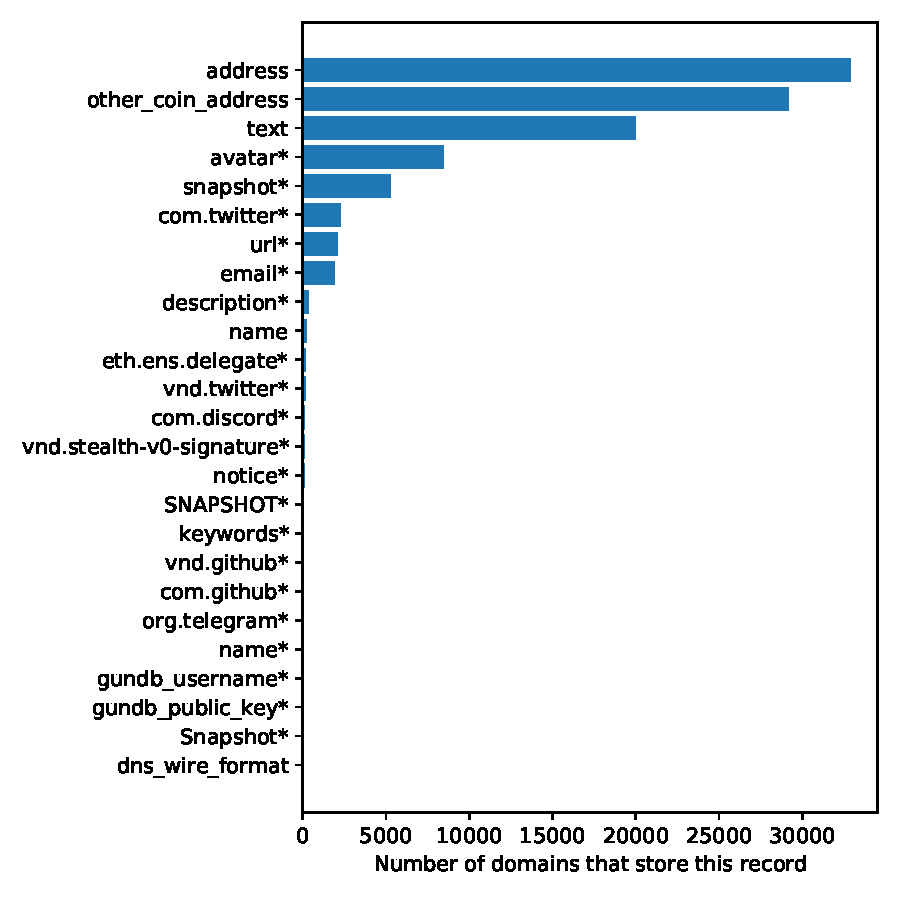
\includegraphics[width=3in]{figs/ens_names.pdf}
	\caption{Records stored by ENS names. *key within ``text'' record}
	\label{fig:ens_records}
\end{figure}

ENS names use smart contracts to fill the roles of the single registrar and 
multiple resolvers in the system. When claiming a name for the first 
time, the user sends a transaction from their wallet to the ENS Registrar 
Controller 
contract, requesting that the name be registered and transferred to the 
ownership of the wallet. The ENS Registrar Controller sets a number of default 
values, including a default wallet 
address record that maps the name to the wallet address that owns it, and a 
default resolver contract for the 
name, which at the moment is the ``ENS Public Resolver 2'' smart 
contract.\footnote{The public 
resolver contract was updated in the past, and almost all ENS names have now 
changed their resolvers 
from the ``Old'' resolvers to the current resolvers.} To fully 
resolve a 
name, a user must first query the ENS Registrar Controller to determine the 
name's designated resolver, and then query that resolver for the record 
associated with the name. Resolver contracts are allowed to access the storage 
of the ENS Registrar Controller, which means they don't have to perform another 
transaction for the resolver to know that a new record has been created by the 
ENS Registrar Controller. 

Users cannot query a resolver for a name's records directly: they must first 
convert the name to its keccak256 hash. These 
name hashes are referred to as ``nodes.'' Because keccak256 hashes are not 
reversible, 
translating a node back to a name requires another contract, the ENS Reverse 
Registrar. Names are not required to have entries in the ENS Reverse Registrar, 
so this contract is not always able to translate a given node 
back to a name. 

One more notable feature of ENS names is that anyone may renew 
them, not just their owners. The reason for this design choice 
is unclear.

To study this ecosystem, we took a sample of names from the eight resolver 
contracts that were set by the most names as their default resolver. We chose 
eight because the distribution of resolvers is long-tailed: the majority of 
resolvers resolve only a few names, while the eight most popular resolvers 
resolve the majority of names. We excluded addresses that were set as resolvers 
by many names but did not implement the ENS resolver specification, under the 
assumption that these were mistakes. Such misconfigured resolver addresses 
include the null address, 
0x0, as well as other smart contracts used by the ENS ecosystem, such as the 
``Base Registrar Implementation.''  The remainder of the resolvers we chose are 
detailed in Table~\ref{tab:ens_resolvers}.

At the time that we performed this study, 667,369 ENS names had been 
registered. Names that did not specify a resolver when they were registered 
were assigned the default ENS Public Resolver 2, which presumably accounts for 
the vast majority of the names that never performed an explicit transaction 
setting their resolver. \randall{I'm in the middle of checking this.} 

Figure~\ref{fig:ens_records} shows the distribution of the types of records 
stored by our sample of names. The majority resolve to wallet addresses or text 
records, not IP addresses, traditional domains, or DS addresses. We broke down 
the text records, which are key/value pairs, by the most common key names: 
these keys are marked with an asterisk. Only the most common 25 keys are shown. 
We note that only 17 names had \texttt{dns\_wire\_format} records, which are 
intended to store traditional DNS 
records, and all 17 are malformed as far as we can tell. \randall{should maybe 
work on that some more? Couldn't tell what was wrong by examining the octets.}

%Describe the registrar/registry/resolver structure. We took a sample 
%of X domains from the most 
%frequently updated resolver contracts.
%
%Haven't found anything bad yet except loli-hentai.x. This 
%system, like all other uncensorable systems, will probably 
%eventually attract CSAM. Describe what we did to find 
%domains, how I crawled a subset.

\subsubsection{Unstoppable Domains}

\begin{figure}[t]
	\centering
	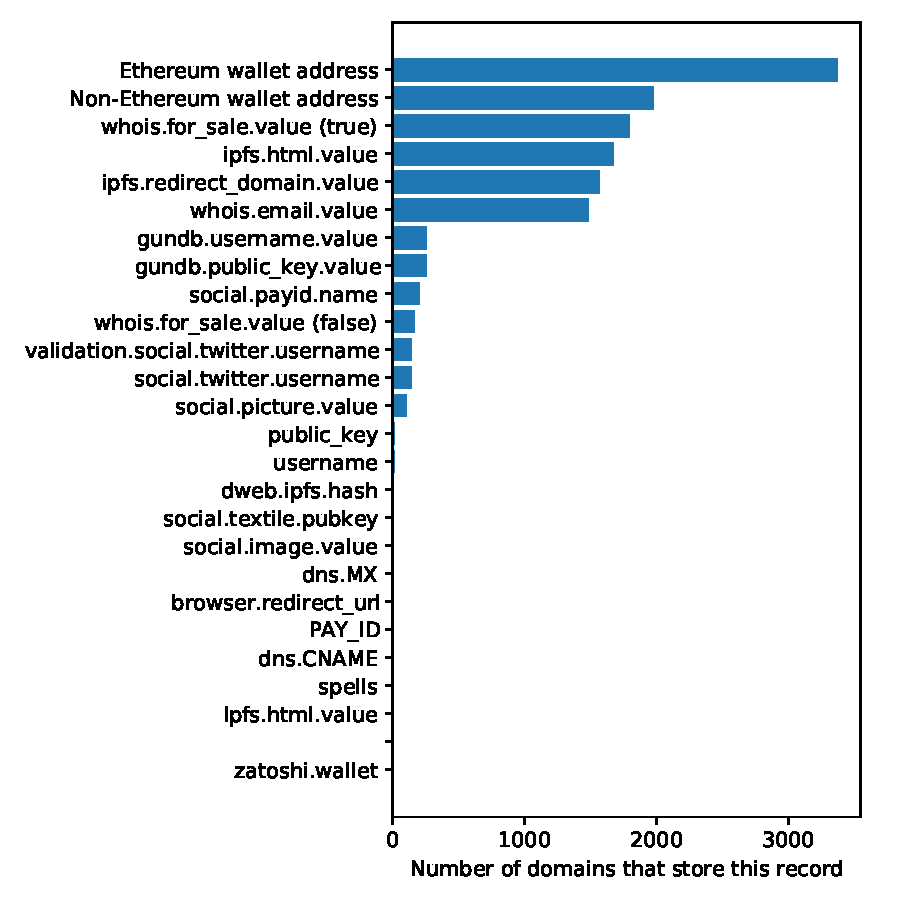
\includegraphics[width=3in]{figs/all_unstoppable_records.pdf}
	\caption{Records stored by Unstoppable Domains names.}
	\label{fig:unstoppable_records}
\end{figure}

%Describe the registry contract and the crawled domains (I did 
%crawl these didn't I?)

Like ENS, Unstoppable Domains uses Ethereum smart contracts as 
registrars. Unstoppable names are divided into two systems. CNS 
(Crypto Name System) contains all names with \texttt{.crypto} 
TLDs, and has separate registry and resolver contracts. This 
system was created first. Later, Unstoppable added UNS 
(Unstoppable Name System), which simplified name resolution by 
combining the resolver and registry contracts, and added several 
new TLDs. Unstoppable names never have to be renewed; they are 
purchased once and then owned for life. This is primarily 
because Unstoppable Domains does not have the capability to 
reclaim a name unless the private key of the owning wallet is 
known to them. 

Unstoppable names are referenced by their namehashes, which are 
similar to ENS's ``nodes.'' We extracted all namehashes from the 
Unstoppable Domains registry contract by searching all of its 
transactions, and then found each name's records by querying the 
Unstoppable metadata endpoint at 
\texttt{https://metadata.unstoppabledomains.com/metadata/}. 
Figure~\ref{fig:unstoppable_records} shows the 
distribution 
of record types found in the Unstoppable Domains names. As in 
ENS, the majority of names have wallet records rather than 
records that point to websites in any way. The next most common 
type of record is ``whois.for\_sale.value,'' showing that many 
names are seen as speculative assets. Unstoppable Domains also 
provides an easy way for users to link to IPFS records. IPFS, 
the ``Inter-Planetary File System,'' is a distributed 
blockchain-based hosting service that allows users to host 
static websites.

We performed a web crawl of all of the Unstoppable names that 
had records pointing to websites, whether IPFS records, 
traditional IP addresses, or traditional domains. We took 
screenshots of the 367 websites we arrived 
at, inspected them manually, and did not find any evidence of 
malware use. Most 
websites were personal sites, Web3-based business sites, or related to the sale 
or collection of NFTs. 

Unstoppable Domains has claimed that their naming system is not well suited for 
malware authors or other miscreants for two reasons. First, Unstoppable 
polices which domains may be sold. The CEO of Unstoppable Domains, Matthew 
Gould, stated in an email that Unstoppable ``prevented the 
registration of domains associated with known pirating software or other types 
of IP theft and fraud''~\cite{pegoraro_blockchain_2021}. Second, Unstoppable 
can also seize a domain if that 
domain is hosted by Unstoppable's custody 
wallet, instead of by a private wallet~\cite{pegoraro_blockchain_2021}. In 
fact, other wallet hosting 
services, such as Coinbase's, 
could presumably also seize wallets that store domains, since the private 
keys of those wallets are 
known to the service. However, we note that seizing hosted wallets may not 
be a reliable 
intervention, because malware authors can evade this tactic by simply using 
self-hosted wallets. 

\subsubsection{Low malware adoption of Ethereum-based naming services}

So far, we have not found evidence that malware authors are 
transitioning to Ethereum-based naming services. We suspect that the high 
cost of creating and modifying names in comparison to naming-specific systems, 
like Namecoin and Emercoin, is a 
factor in the apparent low adoption rate. 


\section{Challenges on naming-specific chains}
%\begin{itemize}
%	\item High txn cost is less of an issue: defenders might 
%	be able to register DGA domains? 
%	\item Blocking the whole thing using antivirus and 
%	middleboxes, or taking the whole thing down, is probably 
%	possible, because there's so few legit users. Even that 
%	one proxy stopped serving access to .bit domains. A 51\% 
%	attack is possible on Namecoin because one pool already 
%	had ~60\% of the hashing power. Also possible just to 
%	blocklist every IP recorded in the chain's domain records.
%\end{itemize}

Naming-specific blockchains, such as Namecoin, Emercoin, and Handshake, 
present 
a different set of tradeoffs for defenders and malware authors. These 
blockchains are created with the sole intention of hosting a naming system. 
With fewer users and correspondingly less demand, these systems' names are 
usually much less expensive than names in Ethereum-based systems. This enables 
malware 
authors to use fast flux or DGA-based strategies, and also may enable 
defenders 
to pre-register domains generated by DGAs. Additionally, low demand for 
these 
services from licit users enables interventions that would cause significant 
collateral damage on more popular blockchains. These interventions include 
blocklisting every record within the chain, blocking access to the chain 
entirely (e.g., from enterprise networks or ISPs' networks), or disabling 
its 
bootstrap nodes to prevent new peers from joining the blockchain.

\subsection{Namecoin and Emercoin}
\begin{table}
	\begin{tabular}{lrr}
		\toprule
		Malware & Domain & Lookups \\
		\midrule
		Gandcrab	&	malwarehunterteam.bit	&	696	\\
			&	politiaromana.bit	&	682	\\
			&	gdcb.bit	&	632	\\
			&	zonealarm.bit	&	1256	\\
			&	ransomware.bit	&	2078	\\
			&	nomoreransom.coin	&	2242	\\
		CHESSYLITE	&	leomoon.bit	&	1870	\\
			&	lookstat.bit	&	1420	\\
			&	sysmonitor.bit	&	1038	\\
			&	volstat.bit	&	910	\\
			&	xoonday.bit	&	1146	\\
		Dofoil	&	vrubl.bit	&	1976	\\
			&	levashov.bit	&	2118	\\
			&	vinik.bit	&	12530	\\
		KPOT Stealer	&	kpotuvorot10.bit	&	3902	\\
			&	star-fox.bit	&	701	\\
		Team9 Loader	&	bestgame.bazar	&	1884	\\
			&	forgame.bazar	&	1730	\\
			&	zirabuo.bazar	&	102	\\
			&	tallcareful.bazar	&	292	\\
			&	coastdeny.bazar	&	278	\\
		BazaLoader	&	acegikbcggin.bazar	&	1092	\\
			&	acegilbcggio.bazar	&	934	\\
		Trojan RTM	&	stat-counter-[0-9]-[0-9].bit	&	20996	\\
		Necurs	&	jfbbrj3bbbd.bit	&	3009	\\
		\bottomrule
	\end{tabular}
	\caption{Examples of malicious Namecoin and Emercoin domains in the October sample of B-root 
	queries. \randall{names need citations?}}
	\label{tab:namecoin_emercoin}
\end{table}

%Plenty of DGA .bit stuff in the b-root leakage, so malware is 
%still using Namecoin for sure. Should check the diffs between 
%the old and new B-root dumps (numbers of hits for each TLD, 
%etc)
%
%Cite/summarize those two papers that found all sorts of 
%nastiness on these chains.

Because blockchain names require alternate resolution systems, we predicted 
that many of them would ``leak'' into the DNS when misconfigured machines 
attempt to resolve them as ordinary DNS domains. An observer might therefore be 
able to see which names are popular by measuring which blockchain names are 
requested through ordinary DNS requests. We took two 24-hour samples of names 
with Namecoin and Emercoin's alternate TLDs that appeared in 
queries to a root DNS server. One of these samples was from October 19, 2021, 
and the other was from April 15, 2022. We examined the names from each sample 
and found ample evidence of names that are likely to be used by malware. We manually inspected 
the Emercoin and Namecoin names with the most queries, and found that the vast majority of the most 
frequently queried names were associated with malware. An example of malware names from the October 
sample of B-root queries is shown in Table~\ref{tab:namecoin_emercoin}. We found that many of the 
names appeared to be randomly generated, making them unlikely to be benign. The only popular Emercoin 
or Namecoin name that was not associated with malware was \texttt{nnm-club.lib}, which appears to be a 
pirating site. These findings are consistent with previous work that found the vast majority of names 
and IPs on Emercoin and Namecoin to be associated with malicious 
behavior~\cite{patsakis_unravelling_2020, casino_unearthing_2021}. \randall{more results from these 
papers?}

%Second, \randall{something about how the domains looked up change over time}.

%Second, we note that some of these names appear to be intended for typo 
%squatting. \randall{Tens of? Hundreds of?} lookups occur for variations of 
%popular names such as ``netflix,'' ``gmail,'' ``apple,'' and 
%``yahoo.'' The string ``netflix'' in particular was popular. \randall{All of these were .kred and 
%.luxe and stuff, not Namecoin/Emercoin.

\subsubsection{Handshake}
\begin{table}
	\begin{tabular}{lr}
		\toprule
		Record & Names with Record \\
		\midrule
		Default NS and GLUE4 records & 102,386 \\
		\hspace*{0.2in} No A records & 102,285\\
		\hspace*{0.2in} A 44.235.163.135 & 94 \\
		\hspace*{0.2in} A 52.43.158.89 & 4 \\
		\hspace*{0.2in} A 144.91.114.245 & 2 \\
		\hspace*{0.2in} A 1.1.1.1 & 1 \\
		Invalid name & 98,068 \\
		No record (null) & 845 \\
		TXT record & 138 \\
		\hspace*{0.2in} ``hello fx-wallet'' & 110 \\
		\hspace*{0.2in} Other & 28 \\
		Non-default NS record & 32 \\
		Non-default GLUE4 record & 11 \\
		Distributed storage address & 7 \\
		\midrule
		Total unique names & 201,458 \\
		Total records & 201,487 \\
		\bottomrule
	\end{tabular}
	\caption{Record types in the Handshake namespace.}
	\label{tab:handshake_records}
\end{table}

Handshake is a new blockchain-based system that aims to 
replace the root DNS 
zone. As such, it offers its users the ability to purchase 
nearly any string to 
use as a TLD. Rather than selling second-level domains 
itself, the Handshake ecosystem purports to allow its users 
to act as registrars who can sell their own domains. 
Handshake's stated goal is not to replace the traditional DNS 
system: Handshake records are designed to store the domains 
and IP addresses of traditional authoritative nameservers, 
rather than to store A, AAAA, or CNAME records. However, we note that nothing 
restricts malware authors from recording the IP addresses of C2 servers as NS 
records, or running an authoritative nameserver and a C2 server on the same 
machine. Handshake also allows users to store TXT records, which can 
contain the addresses for decentralized web hosting systems 
like Skynet or IPFS. Malware users could potentially use 
Handshake as a naming system to find content stored in 
content-addressed distributed storage systems. Additionally, Handshake 
advertises themselves as ``the only naming blockchain with a lightweight 
recursive DNS resolver, which you can easily embed into 
browsers, apps, and devices''~\cite{namebase_access_handshake}. 
This lightweight resolver may be attractive to malware authors because it is 
small enough to use as part of a malware payload.

We collected a sample of approximately 201,000 Handshake names and analyzed the 
records assocated with them. Table~\ref{tab:handshake_records} 
summarizes our findings. At the moment, Handshake names appear to be 
overwhelmingly used as speculative assets. Only 0.14\% of names in our sample 
had records that led to either IP addresses or DS addresses, assuming the 
non-default nameserver and glue records do lead to IP addresses or DS 
addresses. Nearly half of registered Handshake domains cannot be resolved by 
the HNS client, since they contain illegal characters like emojis or are solely 
composed of numbers: these names are nevertheless allowed to be minted.

%Handshake stats:
%\begin{itemize}
%	\item The vast majority of names just have two GLUE4 
%	records with two nameservers: “ns1.name” and “ns2.name”. 
%	The IPs in these glue4 records are 44.231.6.183 and 
%	54.214.136.246, respectively.
%	\item Many of the most expensive TLDs (.x, .crypto, .js, 
%	.8, .wallet) return an SOA record pointing to 
%	``a.misconfigured.powerdns.server''
%	\item ~100K had a nameserver record (all of them pointed 
%	to what I assume is the Namebase resolver, except one or 
%	two.) Out of those 100,000, only 101 actually had an A 
%	record. 94/100 point to one IP address: 44.235.163.135. 
%	That's an AWS IP that gives a 404 if you visit it with a 
%	browser. Four more point to 52.43.158.89 (another AWS 
%	IP), which redirects to an unconfigured distributed 
%	hosting provider site. One points to 1.1.1.1, and two 
%	look like someone's unconfigured personal website.
%\end{itemize}




\section{What might cause a naming system to present a threat?}

Out of the five naming systems we examine, we find none so far that present an 
entirely intractable problem for defenders. For a naming system to present a  
threat, it must be both easily usable by malware authors and 
popular enough that blocking its bootstrap nodes, or blocking 
access to it entirely, will cause significant collateral damage to licit users.
For a system to be widely adopted by licit users, it must have three necessary characteristics. 

First, the system's name management must be as 
easy or easier than name management on traditional DNS domains. Users must not be required to write 
code themselves to interact with smart contracts, as is currently the case with each of the systems we 
study. Users also must not be required to run a blockchain node in order to manage their names, as 
Handshake currently requires to the best of our knowledge.

Second, the transactions that are required to register and update names must be affordable. 
Transactions on Ethereum, in our experience, cost anywhere between \$60 and \$140 during the course of 
our experiments, although we discovered that we were attempting to make transactions during periods of 
high network congestion and fees were unusually high. Even transaction fees as low as ten dollars per 
transaction are far less affordable than transaction fees on naming-specific chains, which can be as 
low as a few cents. This dynamic may make ordinary users more likely to embrace naming systems built 
on naming-specific chains, rather than general-purpose chains. However, general-purpose chains may be 
better known, and therefore more likely to be trusted by users even if transaction fees are higher 
than on naming-specific chains. A trade-off may therefore exist between affordability and perceived 
trustworthiness and name recognition. 

Third, licit users are unlikely to embrace any naming system that does not have widespread browser 
adoption. Browser adoption is hindered by naming systems' lack of coordination, which currently leads 
to name collisions: for example, the alternate TLDs \texttt{.wallet}, \texttt{.coin}, and \texttt{.x} 
are currently used by multiple blockchain naming systems. Some newly created ICANN TLDs also collide 
with Handshake TLDs, such as \texttt{.music}. Naming collisions present a barrier to browser adoption 
because the browser would either have to enforce some sort of precedence for systems that include 
colliding names, or users would have to choose which naming system to use for each name with 
collisions. Either option will confuse and frustrate users who are unfamiliar with the concepts of 
namespaces. So far, only browsers that focus on privacy as one of their primary features have chosen 
to resolve alternate naming systems, and none have chosen to resolve systems that might collide with 
either each other or ICANN TLDs. Until browsers can resolve an alternate naming system natively, users 
are unlikely to adopt that naming system.

%What would cause a decentralized naming system to be popular enough that 
%defenders wouldn't want to block access to it?
%\begin{itemize}
%	\item Ease of use: owners don't have to write code
%	\item Affordable txns
%	\item Widespread browser adoption
%\end{itemize}

\section{Conclusion}

While decentralized naming and hosting systems pose challenges, they cannot 
entirely 
eliminate their reliance on systems with centralized authority. Whenever 
malware uses a centralized 
resource to enable its use of decentralized ones, defenders can intervene. 
Defenders cannot serve 
legal takedown orders to a centralized entity to take 
down a blockchain domain, but they can prevent malware from accessing the 
blockchain in the first 
place, or target the DNS domain or IP address that the blockchain domain 
resolves to. We examined existing blockchain-based naming systems and found that naming specific 
blockchains present a threat, but have been well studied, and are susceptible to defenses such as 
blocklisting every IP address in the system, blocking the proxies that resolve the names, or blocking 
the system entirely, because so little licit 
content exists on those blockchains. We conclude that for a naming system to be truly more dangerous 
than DNS, it must achieve widespread adoption as well as inexpensive transactions and high 
ease-of-use, and no existing naming systems have yet achieved all three characteristics. 

%\section{How big of a threat is blockchain DNS?}
%The original goal of this paper was to say whether malware 
%using blockchain to 
%contact its C\&C servers was actually a huge threat. We can 
%approach this 
%problem in two ways: (1) Map out the ecosystem and say 
%whether it's POSSIBLE, 
%(2) Check the current records being stored and say whether 
%it's already 
%happening.
%
%\section{Whether it's possible}
%
%We haven't yet started up an Ethereum light node to see if 
%it could be part of 
%a malware payload. 
%
%Stefan originally thought that because PCs/phones can't be 
%first class 
%blockchain citizens, malware won't be able to connect to a 
%blockchain without 
%using a proxy. The proxy would be an intervention point for 
%defenders to say, 
%stop serving this stuff, we have a court order. The 
%assumption there is that 
%malware can't connect to a blockchain without using a proxy. 
%I think that's 
%incorrect because the Ethereum nodes themselves use a 
%Chord-like protocol, 
%Kademlia, which I assume-but-need-to-check is a thing where 
%one node knows more 
%nodes, which know more nodes, etc. 
%
%Kademlia relies on bootstrapping, and in fact, the Ethereum 
%nodes out there 
%supposedly get their node lists from a set of bootstrap 
%nodes. You probably 
%can't outright take down the bootstrap nodes, because that 
%breaks new nodes 
%connecting to Ethereum. 
%
%Start with the simplest case - hard-coded Ethereum node 
%domains/IPs. That isn't 
%any better than just having hard coded domains/IPs of your 
%C\&C server, because 
%they're still easy for defenders to block. The caveat is, 
%maybe defenders don't 
%want to take down innocent Ethereum nodes? Because they 
%serve another, benign, 
%purpose besides malware. Stefan thinks defenders wouldn't 
%hesitate to take down 
%nodes that were hard-coded as malware access points to 
%Ethereum. But what if 
%those nodes were the official bootstrap nodes? Defenders 
%wouldn't want to take 
%those down.
%
%\subsection{Light nodes}
%
%Is it enough to just do the PING-PONG and then try to sync 
%txns? I mean, all of 
%that will be much easier if you use a light client, but 
%could you even pull 
%that code out and do it yourself? Or will the full nodes 
%say, nah we don't want 
%to connect to you? 

%Stefan was wondering which Ethereum nodes are actually used 
%for transactions, 
%and whether there's an even distribution or some nodes are 
%taking all the 
%strain. I wonder if you could say, lots of ppl are making 
%txns using Infura's 
%full nodes, let's block those txns from going out onto the 
%network? If no one 
%else can verify them, they can't get added. Or you could 
%DDoS 
%a full node to 
%prevent it sending out the message that says it's mined the 
%next block, but I'm 
%sure someone has thought of that attack already.
%
%\section{Extra interesting stuff we found along the way}
%
%\subsection{Typo squatting}


\bibliographystyle{IEEEtran}
\bibliography{references}

%\appendix
%\section{Ethics}
%
%This work raises no ethical concerns.

\end{document}
